\documentclass{beamer}
\usetheme{simple}
\usepackage[brazil]{babel}
\usepackage[utf8]{inputenc}
\usepackage{lmodern}
\usefonttheme[onlymath]{serif}
\usepackage[scale=2]{ccicons}

\usepackage{graphicx,hyperref,url,pgfplots}
\usepackage{media9}
\usepackage{amsmath} 
\usepackage{array,booktabs}
\usepackage{pdfpages}
\pgfplotsset{compat=1.15}
\pgfplotsset{width=7cm}


\setbeamercovered{invisible}
\newcommand{\pausar}{\pause}
\newcommand{\df}[1]{\,\mathrm{d}#1}
\newcommand{\parcial}[3]{\dfrac{\partial^{#1}#2}{\partial #3^{#1}}}

\usepackage{tikz}
\usepackage{xcolor}
\usetikzlibrary{scopes}
\usepackage{verbatim}
\usetikzlibrary{patterns}
\usepackage{algorithm}
\usepackage{algpseudocode}

\usepackage{listings}
	\definecolor{codegreen}{rgb}{0,0.6,0}
	\definecolor{codegray}{rgb}{0.5,0.5,0.5}
	\definecolor{codepurple}{rgb}{0.58,0,0.82}
	\definecolor{backcolour}{rgb}{0.92,0.92,0.92}
	\lstset{language=Python, 
	backgroundcolor=\color{backcolour},   
	commentstyle=\color{codegreen},
	keywordstyle=\color{magenta},
	numberstyle=\tiny\color{codegray},
	stringstyle=\color{codepurple},
	basicstyle=\fontsize{8}{11}\ttfamily,
	frame=lines,
%	numbers=left,
	tabsize=2,
	morekeywords={models, lambda, forms}}


\title{Filtro de Kalman}
\subtitle{Introdução - Sistemas Lineares}
\date{\today}
\author{Jeferson Lima}
\institute{\url{http://gitlab.com/jeferson.lima}}

\begin{document}

\maketitle

\begin{frame}{Informações Úteis}
	\begin{block}{Material disponível em:}
		\href{Robótica Móvel - Wiki}{https://gitlab.com/cursoseaulas/robotica-movel/-/wikis/home}
	\end{block}
	\pausar
	\begin{block}{Datas Importantes}
		\begin{itemize}
		\item Entrega
		\item Envio
		\end{itemize}
	\end{block}
	\pausar
	\begin{block}{Requisitos da Disciplina}
		\begin{itemize}
		\item Teoria de Controle
		\item Linguagem de Programação - \textbf{Python} ou \textbf{C++}
		\item Eletrônica
		\end{itemize}
	\end{block}
\end{frame}

%-----------------------------------------------------------------

\begin{frame}{Teorema de Bayes}
    \framesubtitle{Revisão} {Revisão}
  \begin{itemize}
    \item Estado Estimado $x$ de um sistema observado $z$ e com controle em $u$.
    \item Objetivo:
  \end{itemize}

  \begin{equation}
    P(x|z,u)
  \end{equation}
\end{frame}


\begin{frame}{Bayes Filter}
    \framesubtitle{Revisão}
    
    \begin{block}{}
        \begin{equation*}
            \text{Bel}(x_t) = \eta P(z_t| x_t) \int P(x_t| u_t, x_{t-1}) \text{Bel}(x_{t-1})\text{d}x_{t-1}
        \end{equation*}
    \end{block}

    \begin{itemize}
        \item Predição:
        
        \begin{equation*}
            \overline{\text{Bel}}(x_t) = \int P(x_t| u_t, x_{t-1}) \text{Bel}(x_{t-1})\text{d}x_{t-1}
        \end{equation*}

        \item Correção:

        \begin{equation*}
            \text{Bel}(x_t) = \eta P(z_t| x_t) \int P(x_t| u_t, x_{t}) \overline{\text{Bel}}(x_{t})\text{d}x_{t-1}
        \end{equation*}
    \end{itemize}
\end{frame}


\begin{frame}{Distribuição Normal (Gaussiana)}
    \framesubtitle{Revisão}  
    \begin{itemize}
        \item \textbf{Uma Variável:} $\color{blue}{P(x) \sim N(\mu, \sigma^2)}$
    \end{itemize}

    \begin{block}{}
        \begin{equation*}
            P(x) = \dfrac{1}{\sqrt{2\pi\sigma^2}}\cdot 
        \exp\left\{-\frac{(x-\mu)^2}{2\sigma^2}\right\}
        \end{equation*}
    \end{block}

    \centering
    \begin{tikzpicture}[
    declare function={
      normalpdf(\x,\mu,\sigma)=
      (2*3.1415*\sigma^2)^(-0.5)*exp(-(\x-\mu)^2/(2*\sigma^2));
    },
    hplot/.style={ycomb, mark=o, dashed}, ,scale=0.8]
  
    \begin{axis}[
      width=12cm, height=6cm,
      samples=50,
      xlabel=$x$, ylabel=$p(x)$,
      xlabel style={at={(1,0)}, anchor=north west},
      ylabel style={rotate=-90, at={(0,1)}, anchor=south east},
      legend style={draw=none, fill=none},
      domain=-6:9,
      legend cell align=left,
      xmin=-7, xmax=11]
  
      \addplot [smooth, thick] {normalpdf(x,0,1)}
      node[pos=0.47, pin={right:$\mu=0,\sigma^2=1$}] {};
      \addplot [smooth, blue] {normalpdf(x,0,2)}
      node[pos=0.6, pin={45:$\mu=0,\sigma^2=2$}] {};
      \addplot [smooth, red] {normalpdf(x,-2,1)}
      node[pos=0.25, pin={[text centered, text width=8ex]
        200:$\mu=-1$, $\sigma^2=1$}] {};
  
      \addplot [hplot, samples at={0}] {normalpdf(x,0,1)};
      \addplot [hplot, samples at={0}, blue] {normalpdf(x,0,2)};
      \addplot [hplot, samples at={-2}, red] {normalpdf(x,-2,1)};
  
      \node[anchor=north east] at (axis description cs: 0.975,  0.95)
      {$p(x) = \dfrac{1}{\sqrt{2\pi\sigma^2}}\cdot 
        \exp\left\{-\frac{(x-\mu)^2}{2\sigma^2}\right\}$};
  
    \end{axis}
  \end{tikzpicture}
\end{frame}


\begin{frame}{Distribuição Normal (Gaussiana)}
    \framesubtitle{Revisão}
    \begin{itemize}
        \item Bivariável: $\color{blue}{P(\mathbf{x}) \sim N(\mu, \sum)}$
    \end{itemize}
    \centering
    \pgfplotsset{%
  colormap={whitered}{color(0cm)=(white);
  color(1cm)=(orange!75!red)}
}
\begin{tikzpicture}[
  declare function = {mu1=1;},
  declare function = {mu2=2;},
  declare function = {sigma1=0.5;},
  declare function = {sigma2=1;},
  declare function = {normal(\m,\s)=1/(2*\s*sqrt(pi))*exp(-(x-\m)^2/(2*\s^2));},
  declare function = {bivar(\ma,\sa,\mb,\sb)=
    1/(2*pi*\sa*\sb) * exp(-((x-\ma)^2/\sa^2 + (y-\mb)^2/\sb^2))/2;},scale=0.6]
  \begin{axis}[
    colormap name  = whitered,
    width          = 15cm,
    view           = {45}{65},
    enlargelimits  = false,
    grid           = major,
    domain         = -1:4,
    y domain       = -1:4,
    samples        = 26,
    xlabel         = $x_1$,
    ylabel         = $x_2$,
    zlabel         = {$P$},
    colorbar,
    colorbar style = {
      at     = {(1,0)},
      anchor = south west,
      height = 0.25*\pgfkeysvalueof{/pgfplots/parent axis height},
      title  = {$P(x_1,x_2)$}
    }
  ]
    \addplot3 [surf] {bivar(mu1,sigma1,mu2,sigma2)};
    \addplot3 [domain=-1:4,samples=31, samples y=0, thick, smooth]
      (x,4,{normal(mu1,sigma1)});
    \addplot3 [domain=-1:4,samples=31, samples y=0, thick, smooth]
      (-1,x,{normal(mu2,sigma2)});

    \draw [black!50] (axis cs:-1,0,0) -- (axis cs:4,0,0);
    \draw [black!50] (axis cs:0,-1,0) -- (axis cs:0,4,0);

    \node at (axis cs:-1,1,0.18) [pin=165:$P(x_1)$] {};
    \node at (axis cs:1.5,4,0.32) [pin=-15:$P(x_2)$] {};
  \end{axis}
\end{tikzpicture}
\end{frame}



\begin{frame}{Distribuição Normal (Gaussiana)}
    \framesubtitle{Revisão}
    \begin{itemize}
        \item Bivariável: $\color{blue}{p(\mathbf{x}) \sim N(\mu, \sum)}$
    \begin{equation*}
        P(\mathbf{x}) = \frac{1}{(2\pi)^{\frac{d}{2}\|\sum\|^{\frac{1}{2}}}}\exp\left\{-\frac{1}{2} (\mathbf{x}-\mu)^T\sum{}^{-1}(\mathbf{x}-\mu)\right\}
    \end{equation*}
    
    \item Para um sistema de duas Variável:
    
    \begin{equation*}
        p(\mathbf{x}) \sim N(\mu, \sum)
    \end{equation*}
    logo:     
    \begin{equation*}
        \begin{pmatrix}
            X_1 \\
            X_2
        \end{pmatrix}  \sim \mathcal{N} \left( \begin{pmatrix}
            \mu_1 \\
            \mu_2
        \end{pmatrix} , \begin{pmatrix}
            \sigma^2_1 &  \rho \sigma_1 \sigma_2 \\
            \rho \sigma_1 \sigma_2 &  \sigma^2_2
        \end{pmatrix} \right)
    \end{equation*}
    \end{itemize}
\end{frame}


\begin{frame}{Distribuição Normal (Gaussiana)}
    \framesubtitle{Propriedades}
    \begin{itemize}
        \item Caso Univariavel:
    \end{itemize}
    \centering
    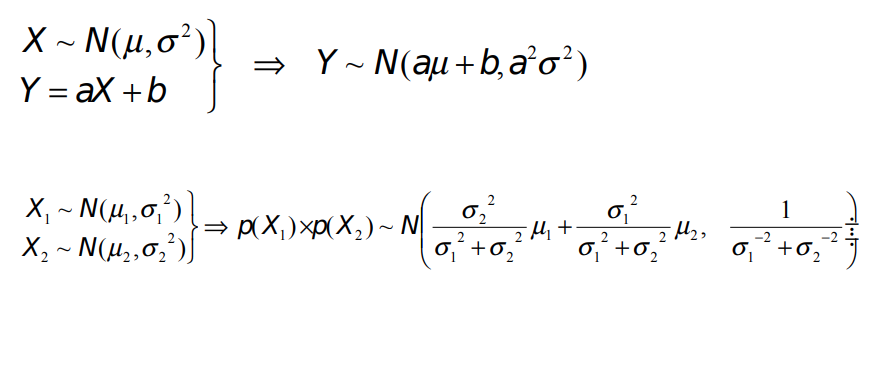
\includegraphics[width=0.8\textwidth]{images/tmp0.png}
\end{frame}


\begin{frame}{Distribuição Normal (Gaussiana)}
    \framesubtitle{Propriedades}
    \begin{itemize}
        \item Caso Multivariável:
    \end{itemize}
    \centering
    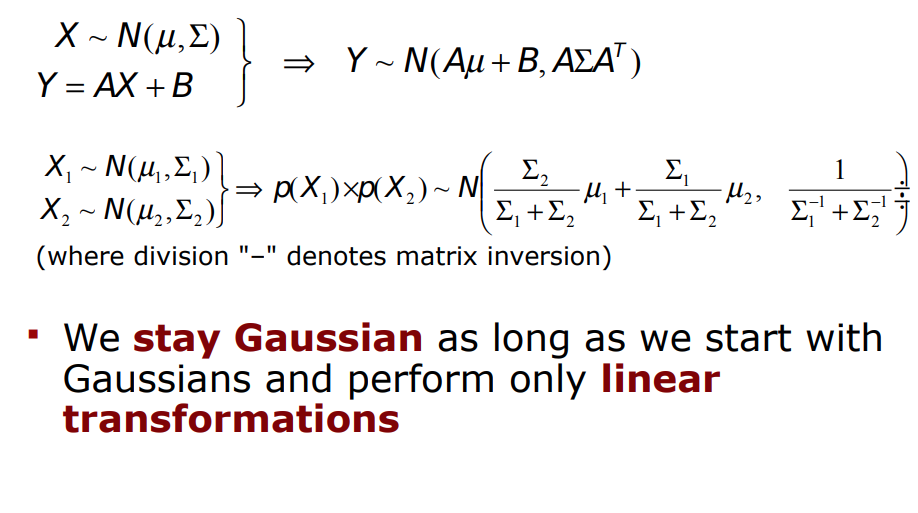
\includegraphics[width=0.8\textwidth]{images/tmp1.png}
\end{frame}




\begin{frame}{Kalman filter}
    \framesubtitle{Modelo determinísticoe estocástico}
    \begin{itemize}
        \item Num modelo determinístico o resultado do sistema é pré determinado em função dos dados de entrada, exemplo:
        \begin{align*} 
            x_t &= A_t x_{t-1} + B_t u_t\\ 
            z_t &= C_t x_t
        \end{align*}

        \item Num modelo estocástico o Resultado do sistema não depende somente dos dados de entrada, mas também de outros fatores, normalmente
        aleatórios:
        \begin{align} 
            x_t &= A_t x_{t-1} + B u_t +  \varepsilon_t\\ 
            z_t &= C_t x_t + \delta_t
        \end{align}

        \begin{itemize}
            \item $A_t$ Matriz $(n \times n)$ que descreve os estados do modelo.
            \item $B_t$ Matriz $(n \times l)$ que descreve os estados do controle.
            \item $C_t$ Matrix $(k\times n)$ sendo os estados de $x_t$.
            \item $ \varepsilon_t$ Variável aleatória do processo.
            \item $\delta_t$ Rúido aleatório com distribuição normal e covariância de $R_t$ e $Q_t$.
        \end{itemize}
    \end{itemize}
\end{frame}


\begin{frame}{Kalman filter}
    \framesubtitle{Representação Grafica}
      \begin{tikzpicture}[
    declare function={
      normalpdf(\x,\mu,\sigma)=
      (2*3.1415*\sigma^2)^(-0.5)*exp(-(\x-\mu)^2/(2*\sigma^2));
    },
    hplot/.style={ycomb, mark=o, dashed}, ,scale=0.8]
  
    \begin{axis}[
      width=8cm, height=5.5cm,
      samples=50,
      legend style={draw=none, fill=none},
      domain=-6:9,
      legend cell align=left,
      xmin=-7, xmax=11]
  
      \addplot [smooth, thick, red] {normalpdf(x,-2,2)} node[] {};
    \end{axis}
  \end{tikzpicture}
  \pausar
  \begin{tikzpicture}[
    declare function={
      normalpdf(\x,\mu,\sigma)=
      (2*3.1415*\sigma^2)^(-0.5)*exp(-(\x-\mu)^2/(2*\sigma^2));
    },
    hplot/.style={ycomb, mark=o, dashed}, ,scale=0.8]
  
    \begin{axis}[
      width=8cm, height=5.5cm,
      samples=50,
      legend style={draw=none, fill=none},
      domain=-6:9,
      legend cell align=left,
      xmin=-7, xmax=11]
  
      \addplot [smooth, thick, red] {normalpdf(x,-2,2)} node[] {};
      \addplot [smooth, black] {normalpdf(x,0,2)} node[] {};
    \end{axis}
  \end{tikzpicture}

  \pausar

\begin{columns}

  \begin{column}{0.5\textwidth}

    \begin{tikzpicture}[
      declare function={
        normalpdf(\x,\mu,\sigma)=
        (2*3.1415*\sigma^2)^(-0.5)*exp(-(\x-\mu)^2/(2*\sigma^2));
      },
      hplot/.style={ycomb, mark=o, dashed}, ,scale=0.8]
    
      \begin{axis}[
        width=8cm, height=5.5cm,
        samples=50,
        legend style={draw=none, fill=none},
        domain=-6:9,
        legend cell align=left,
        xmin=-7, xmax=11]
    
        \addplot [smooth, thick, red] {normalpdf(x,-2,2)} node[] {};
        \addplot [smooth, black] {normalpdf(x,0,2)} node[] {};
        \addplot [smooth, blue] {normalpdf(x,-1,0.6)} node[] {};
      \end{axis}
    \end{tikzpicture}
  \end{column}

  \pausar

  \begin{column}{0.5\textwidth}
      Como encontrar a solução para o grafico azul?

      \pausar
        $\color{blue}{p(x_t|z_{t}, u_t)}  \color{gray}{=\eta} \color{red}{p(z_t| x_t)}\color{black}{p(x_t| z_{t-1}, u_t)}$

        onde:
        \begin{tabular}{l  l}
          $z_t$: & estado observado no tempo $t$\\ 
          $u_t$: & ação no tempo $t$\\
          $x_t$: & estado do sistema em $t$        
        \end{tabular}
    
  \end{column}
\end{columns}
\end{frame}

\begin{frame}{Kalman filter}
    \framesubtitle{Revisão}

    \setlength\extrarowheight{5pt}
        \begin{tabular}{r l}
            $\color{blue}{\text{Bel}}(x_t)$ & = $P(x_t| u_1, z_1,  \cdots, z_t)$ \\
            Bayes & = $\eta P(z_t|x_t,  u_1, z_1,  \cdots,  u_t)P(x_t, u_1, z_1, \cdots, u_t)$ \\
            Markov & = $\eta P(z_t|x_t)P(x_t, u_1, z_1, \cdots, u_t)$ \\
            Prob. Total & = $\eta P(z_t|x_t)\displaystyle\int P(x_t| u_1, z_1, \cdots, u_t,x_{t-1})$ \\
                        &  \quad \quad \quad $P(x_{t-1}| u_1, z_1, \cdots, u_t)\text{d}x_{t-1}$\\
            Markov & = $\eta P(z_t|x_t)$ $\displaystyle\int P(x_t| u_t,x_{t-1})P(x_{t-1}| u_1, z_1, \cdots, u_t)\text{d}x_{t-1}$ \\
            Markov & = $\eta P(z_t|x_t)$ $\displaystyle\int P(x_t| u_t,x_{t-1})\color{blue}{P(x_{t-1}| u_1, z_1, \cdots, z_{t-1}})\color{gray}{\text{d}x_{t-1}}$ \\
        \end{tabular}   
    \begin{block}{Bayes Filter}
        \begin{equation*}
            \color{blue}{\text{Bel}}(x_t)  \color{gray}{=\eta P(z_t|x_t)\displaystyle\int P(x_t| u_t,x_{t-1})}\color{blue}{\color{blue}{\text{Bel}}(x_{t-1})}\color{gray}{)\text{d}x_{t-1}}
        \end{equation*}
    \end{block}
\end{frame}


\begin{frame}[c]{Kalman filter}
    \framesubtitle{Algoritmo}

    \begin{itemize}
        \item Iniciando as Variável:
        \begin{equation}
            \text{Bel}(x_0) = N\left(x_0, \mu_o, {\sum} _0\right)
        \end{equation}
        \item Tempo de convergência do filtro.
    \end{itemize}
\end{frame}

\begin{frame}[c]{Kalman filter}
    \framesubtitle{Algoritmo}
    \begin{itemize}
        \item Com base na equação:
        \begin{equation*}
            \color{blue}{\text{Bel}}(x_t)  \color{gray}{=\eta P(z_t|x_t)\displaystyle\int P(x_t| u_t,x_{t-1})}\color{blue}{\color{blue}{\text{Bel}}(x_{t-1})}\color{gray}{)\text{d}x_{t-1}}
        \end{equation*}
        \item E considerando que o sistema abaixo é linear e observável:
        \begin{equation*}
            \begin{split}
                x_t &= A_t x_{t-1} + B_t u_t\\ 
                z_t &= C_t x_t
            \end{split}
        \end{equation*}
        \item Um sistem é observável se o posto da matriz $\mathcal {O}$ é igual a $n$.
        \begin{equation*}
            \mathcal {O}={\begin{bmatrix}C_t\\C_tA_t\\C_tA^{2}_t\\\vdots \\C_tA^{n-1}_t\end{bmatrix}, \quad \text{rank}(\mathcal {O}}) = n
        \end{equation*}
    \end{itemize}
\end{frame}


\begin{frame}[c]{Kalman filter}
    \framesubtitle{Algoritmo - Prediction}
    \begin{itemize}
        \item Temos a função de probabilidade do sistema, expressa por:
        \begin{equation*}
            p(x_t| u_t, x_{t-1})= N\left(x_t; A_tx_{t-1}+ B_tu_t, Q_t\right)
        \end{equation*}   
        \item ou seja:
        \begin{equation*}
            \overline{\text{Bel}}(x_t)  = \displaystyle\int\underbrace{P(x_t|u_t, x_{t-1})}_{\sim N\left(x_t; A_t x_{t-1}+ B_tu_t, Q_t\right)} \overbrace{\text{Bel}(x_{t-1})}^{\sim N\left(x_{t-1}; \mu_{t-1}, \sum {}_{t-1}\right)}\text{d}x_{t-1}
        \end{equation*}
    \end{itemize}
\end{frame}


\begin{frame}[c]{Kalman filter}
    \framesubtitle{Algoritmo - Prediction}
    \begin{tabular}{p{1.5cm} l l}
        $\overline{\text{Bel}}(x_t)$  & = $\displaystyle\int P(x_t|u_t, x_{t-1})$ & $\text{Bel}(x_{t-1})\text{d}x_{t-1}$ \\
        & \quad\quad\quad\quad\quad $\Downarrow$ & \quad\quad\quad$\Downarrow$ \\
        & $\sim N\left(x_t; A_t x_{t-1}+ B_tu_t, Q_t\right)$ & $\sim N\left(x_{t-1}; \mu_{t-1}, \sum {}_{t-1}\right)$ \\
        & \quad\quad\quad\quad\quad $\Downarrow$ & \\
    \end{tabular}

    \begin{block}{Relembrando ...}
        \begin{equation*}
            P(\mathbf{x}) = \frac{1}{(2\pi)^{\frac{d}{2}\|\sum\|^{\frac{1}{2}}}}\exp\left\{-\frac{1}{2} (\mathbf{x}-\mu)^T\sum{}^{-1}(\mathbf{x}-\mu)\right\}
        \end{equation*}        
    \end{block}

    \begin{tabular}{p{1.2cm} l}
        & $\quad\quad\quad\quad\quad \Downarrow$\\
        $\overline{\text{Bel}}(x_t)$  & = $\eta \displaystyle\int \exp\left\{  -\frac{1}{2} \left(x_t - A_t x_{t-1} - B_t\right)^T Q_t \left(x_t - A_t x_{t-1} - B_t\right)  \right\}$ \\
    \end{tabular}
        
    \begin{tabular}{p{2.3cm} l}
        & $\exp\left\{ -\displaystyle\frac{1}{2} \left(x_{t-1} - \mu_{t-1}\right)^T \sum {}_{t-1} \left(x_{t-1} - \mu_{t-1}\right)  \right\}\text{d}x_{t-1}$
    \end{tabular}    

\end{frame}



\begin{frame}[c]{Kalman filter}
    \framesubtitle{Algoritmo - Prediction}

    \begin{itemize}
        \item Continuando ...
    \end{itemize}

    \begin{tabular}{p{1.2cm} l}      
        $\overline{\text{Bel}}(x_t)$  & = $\eta \displaystyle\int \exp\left\{  -\frac{1}{2} \left(x_t - A_t x_{t-1} - B_t\right)^T Q_t \left(x_t - A_t x_{t-1} - B_t\right)  \right\}$ \\
    \end{tabular}
        
    \begin{tabular}{p{2.3cm} l}
        & $\exp\left\{ -\displaystyle\frac{1}{2} \left(x_{t-1} - \mu_{t-1}\right)^T \sum {}_{t-1} \left(x_{t-1} - \mu_{t-1}\right)  \right\}\text{d}x_{t-1}$
    \end{tabular}    

    \begin{block}{Prediction}
        \begin{equation}
            \overline{\text{Bel}} = 
            \left\{
            \begin{aligned}
                    \overline{\mu}_t & = A_t\mu_{t-1} + B_t u_t\\
                    \overline{\sum}_t & = A_t {\sum}_{t-1} A_t^T+ Q_t\\
            \end{aligned} \right.
        \end{equation}
    \end{block} 
\end{frame}


\begin{frame}[c]{Kalman filter}
    \framesubtitle{Algoritmo - Measurement Update}
    \begin{itemize}
        \item Considerando a saída do sistema:
        \begin{equation*}
            z_t = C_t x_t + \delta_t
        \end{equation*}
        \item Apresentadas as equações lineares do observador de estados, temos a função de probalilidade:
        \begin{equation*}
            P(z_t| x_t)= N\left(z_t; C_t x_t, R_t\right)
        \end{equation*}   
        \item ou seja:
        \begin{equation*}
            \text{Bel}(x_t)  = \eta \underbrace{P(z_t|x_t)}_{\sim N\left(z_t; C_t x_t, Q_t^{-1}\right)} \overbrace{\overline{\text{Bel}}(x_t)}^{\sim N\left(x_t; \overline{\mu}_t, \overline{\sum}_t\right)}
        \end{equation*}
    \end{itemize}
\end{frame}


\begin{frame}[c]{Kalman filter}
    \framesubtitle{Algoritmo -  Measurement Update}
    \begin{tabular}{p{1.5cm} l l l}
        $\text{Bel}(x_t)$  & = $\eta$ & $P(z_t| x_t)$ & $\overline{\text{Bel}}(x_t)$ \\
        & & $\quad \Downarrow$ & $\quad\Downarrow$ \\
        & & $\sim N\left(z_t; C_t x_t, Q_t\right)$ & $\sim N\left(x_t; \overline{\mu}_t, \overline{\sum}_t\right)$ \\
        & & $\quad \Downarrow$ &  \\
    \end{tabular}

   \begin{tabular}{p{1.5cm} l l}
        $\text{Bel}(x_t)$  & = $\eta$ & $\exp\left\{  -\displaystyle\frac{1}{2} \left(z_t - C_t x_t\right)^T R_t \left(z_t - C_t x_t\right)  \right\}$ \\
    \end{tabular}
    
    \begin{tabular}{p{2.5cm} l}
        & $\exp\left\{ -\displaystyle\frac{1}{2} \left(x_t - \overline{\mu}_t\right)^T \overline{\sum}_t^{-1} \left(x_t - \mu_t\right) \right\}$
    \end{tabular}  

    \begin{block}{Measurement Update}
        \begin{equation}
            \overline{\text{Bel}} = 
            \left\{
            \begin{aligned}
                    \mu_t & = \overline{\mu}_t + K_t(z_t -C_t \overline{\mu}_t)\\
                    \sum_t & = (I-K_tC_t)\overline{\sum}_t \\
            \end{aligned} \right.
        \end{equation}

        \begin{equation}
            \text{Com }
            K_t = \overline{\sum}_tC_t^T(C_t\overline{\sum}_tC_t^T+R_t)^{-1}
        \end{equation}
    \end{block} 
\end{frame}



\begin{frame}[c]{Kalman filter}
    \framesubtitle{Algoritmo}
    \begin{algorithm}[H]
        \caption{Kalman-filter}
        \label{array-sum}
        \begin{algorithmic}[1]
        \Procedure{Prediction}{$\mu_{t-1}, {\sum}_{t-1}, u_t, z_t$}
            \State $\overline{\mu}_t = A_t\mu_{t-1} + B_t u_t$
            \State $ \overline{\sum}_t = A_t {\sum}_{t-1} A_t^T+ Q_t$ 
            \State \textbf{Return} $\left(\overline{\mu}_t, \overline{\sum}_t\right)$
        \EndProcedure
        \Procedure{MeasurementUpdate}{$A$}
            \State $K_t = \overline{\sum}_tC_t^T(C_t\overline{\sum}_tC_t^T+R_t)^{-1}$
            \State $\mu_t  = \overline{\mu}_t + K_t(z_t -C_t)$
            \State{$\sum_t = (I-K_tC_t)\overline{\sum}_t$}
            \State \textbf{Return} $\left(\mu_t, \sum_t\right)$
        \EndProcedure
        \end{algorithmic}
    \end{algorithm}
\end{frame}



\begin{frame}[c]{Kalman filter}
    \framesubtitle{Exercício}
\end{frame}


\begin{frame}[c]{Kalman filter}
    \framesubtitle{Desafio Carro Autonomo x Ciclista}
\end{frame}



% \begin{frame}{Extended Kalman filter}

% \end{frame}

\begin{frame}[t]{Referências}
    \begin{itemize}
        \item http://www.embarcados.com.br/arduino-entradasaidas-digitais/
        \item \href{https://www.youtube.com/watch?v=DE6Jn2cB4J4&list=PLgnQpQtFTOGQrZ4O5QzbIHgl3b1JHimN_&index=5}{aula kalman} 
        \item \href{https://www.youtube.com/watch?v=QZ5q59H2qaI}{Fusion Odometry and IMU}
        \item http://www.ic.uff.br/~bianca/ia-20091/aulas/IA-Aula11.ppt (crença)
    \end{itemize}
\end{frame}
\end{document}



% % https://classroom.udacity.com/courses/ud810/